%!TEX root = ../thesis.tex

\chapter{Umsetzung}
\label{chap:coding}
In diesem Kapitel wird auf den Aufbau der Implementierung eingegangen. Zunächst ein allgemeiner Überblick über das Vorgehen. Dies wird im folgenden als Pipeline bezeichnet und wird im \prettyref{sec:pipeline} allgemein erkläutert.

Nachdem ein genereller Überblick über die einzelnen Bestandteile gegeben wurde wird auf die einzelnen Schritte der Pipeline genauer eingegangen.
Anfänglich werden einmalige Vorbereitungsschritte aufgeschlüsselt, hierzu gehört zu einem großen Teil die Kalibrierung der genutzten Kamera in \prettyref{sec:camera} und die Bestimmung der Charakteristika dieser. 

Darauf folgt in \prettyref{sec:board} die Kalibrierung und die Erkennung der Felder des Dartboardes. Es werden verschiedene getestete Ansätze erörtert und ihre Vor- und Nachteile dargestellt.

Des Weiteren werden die einzelnen Abschnitte der Pipeline näher beleuchtet und auf die Implementierung und das Vorgehen eingegangen. Dies umfasst von der Segmentierung der Dinge, die nicht zum Dartboard gehören in \prettyref{sec:segmentation}. Bis hin zur konkreten Bestimmung der erzielten Punktzahl in \prettyref{sec:score}. 
\todo{Umsetzung einteilen und implementieren}
       
\section{Pipeline Überblick}
\label{sec:pipeline}
\begin{itemize}
\item Einmalige Schritte erläutern
\item Unterteilung der Einzelnen Threads
\item Blob Storage
\item zweiter Thread Pfeil aus Blob
\item Punktzahl Speicher
\end{itemize}
Ein genereller Überblick über die Pipeline wird in Abbildung \prettyref{Fig:pipeline} gegeben. Zu erkennen ist, dass es zwei sich wiederholende Teile gibt. Als Verbindungsglied zwischen diesen steht der Contour Storage. Dieser speichert Informationen zu jedem aufgenommenen Bild. Auf den Storage, seine Funktionsweise und die weitere Verarbeitung wird in \prettyref{sec:foreground} eingegangen. 

Am Anfang der Pipeline steht die generelle Kalibrierung der Kamera, diese gehört nur bedingt zur Pipeline hinzu. Die Kamera Kalibrierung muss für eine spezifische Kamera nur ein einziges mal ausgeführt werden, abgesehen von dem Fall, dass die Kamera eine Fokussierung besitzt. In diesem Fall muss dieser Schritt nach jedem Fokus Vorgang erneut ausgeführt werden. Auf die Kalibrierung der Kamera wird im einzelnen in \prettyref{sec:camera} eingegangen.

Ist die generelle Kalibrierung abgeschlossen, können die hieraus gewonnenen Informationen genutzt werden, um das Dartboard und dessen Felder zu segmentieren und unterscheiden zu können. Das Resultat dieser Kalibrierung ist eine Funktion, die eine Abbildung von einem Pixel zu einer spezifischen Punktzahl auf dem Dartboard darstellt. In \prettyref{sec:board} wird genauer beschrieben, welche Ansätze zu diesem Zweck verfolgt wurden und wie die letztendliche Umsetzung vorgenommen wurde.
\begin{figure}
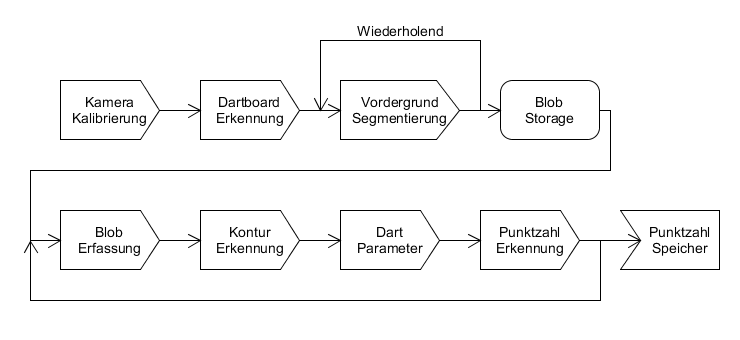
\includegraphics[width=\textwidth]{media/pipeline.png}\\
\caption{\textbf{Übersicht der einzelnen Schritte}}
\label{Fig:pipeline}
\end{figure}

\section{Kamera Kalibrierung}
\label{sec:camera}
Um genauere und bessere Daten aus der Kamera ziehen zu können müssen vorher einige Parameter bestimmt werden. Im \prettyref{sec:basics} wurde bereits das Kamera Modell erläutert. 
Zur Bestimmung der erwähnten Parameter. \textquote{Camera calibration is a necessary step in 3D computer vision in order to extract metric information
from 2D images.} \autocite[5]{Zhang2000}

\section{Erkennung des Dartboards}
\label{sec:board}
Stage 1 Board finden:
     mehrere Ansätze
     Blobs des boardes erkennen
     Felder Kanten erkennen
     Board Kalibrieren als Erweiterung der Kamera Kalibrierung
        
        Dartboard Koordinaten bestimmen im Verhältnis zur Kamera.
       Eigentliche Kalibrierung via klicken,
       wie viele Punkte sind nötig


\section{Segmentierung des Vordergrundes}
\label{sec:segmentation}
Stage 3 Vordergrund von Hintergrund trennen
Foreground detection naiver Ansatz und Algorithmen
Parameter Erklärung
Vereinfachung und Annahmen
Aufgetretene Problematik
\section{Verarbeitung der Vordergrundinformationen}
\label{sec:foreground}
Stage 4 Im Extrahierten Vordergrund entscheiden was Pfeil ist
\section{Punktzahlbestimmung}
\label{sec:score}
Stage 5 Parameter vom Pfeil bestimmen(Spitzen)
